\section{Experiments}
\label{sec:experiments}

All reported numbers are generated by repository scripts. The original full run uses $64$ replicates per grid cell and candidate counts $N \in \{1,2,4,8,16,32,64\}$. The expanded v3 suite adds candidate-count stress to $N=256$, target-overshoot sweeps, a high-$N$ repair ladder, pilot-label budget ablations, and rollout-noise stress. We organize the evidence around six reviewer questions.

\subsection{Does candidate-count pressure improve proxy return while harming real utility out of support?}

Yes, in the controlled out-of-support condition. Table~\ref{tab:headline} shows the phase split. In support and at the support edge, naive top-score selection improves selected real utility. Out of support, it improves the proxy score but decreases real utility.

\begin{table}[t]
\centering
\small
\caption{\textbf{Naive top-score selection phases.} The same selection rule helps under supported targets and hurts under the out-of-support target. Values are means across replicates.}
\label{tab:headline}
\begin{tabular}{lrrrrl}
\toprule
Target & Support gap & $\score_{N=1}$ & $\score_{N=64}$ & $\utility_{N=1}\rightarrow\utility_{N=64}$ & Phase \\
\midrule
In support & 0.000 & 4.821 & 4.978 & $4.821 \rightarrow 4.975$ & helps \\
Edge support & 0.000 & 6.312 & 6.478 & $6.311 \rightarrow 6.454$ & helps \\
Out of support & 3.000 & 9.299 & 9.468 & $7.825 \rightarrow 7.381$ & hurts \\
\bottomrule
\end{tabular}
\end{table}

The failure is not a mere lack of prompt satisfaction. For the out-of-support target $\tau=9.314$, selected proxy return is already close to the prompt at $N=1$ and becomes larger as $N$ grows. What changes is the tail: the selected risk rises from $0.0123$ to $0.0174$, behavior log-likelihood falls from $-4.888$ to $-5.325$, and real utility drops by $0.444$. Figure~\ref{fig:fantasy} visualizes this divergence.

\begin{figure}[t]
  \centering
  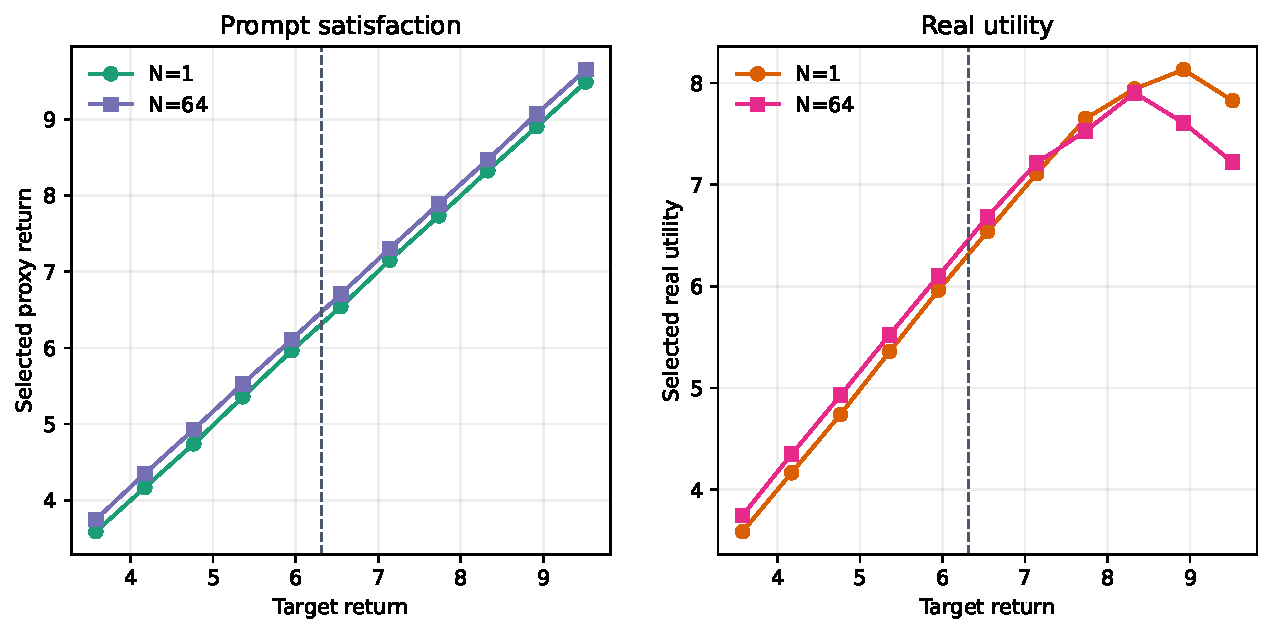
\includegraphics[width=0.92\linewidth]{figures/target_return_sweep.pdf}
  \caption{\textbf{Target-return sweep from the original suite.} At low and supported target returns, increasing $N$ generally improves real utility. As the requested return moves beyond support, the $N=64$ real-utility gain turns negative even though proxy return remains high.}
  \label{fig:sweep}
\end{figure}

The sweep in Figure~\ref{fig:sweep} shows the transition across target returns. For example, at target $7.733$ the $N=64$ real-utility gap is $-0.123$; at target $8.920$ it is $-0.523$; at target $9.514$ it is $-0.604$. This is the empirical Tail Phase Diagram: the sign of the candidate-count effect changes as support gap grows.

\subsection{Does the failure persist to \texorpdfstring{$N=256$}{N=256}?}

The expanded v3 suite extends the out-of-support candidate-count tail to $N=256$. Table~\ref{tab:tail256} shows the result. Selected proxy return rises from $9.283$ at $N=1$ to $9.507$ at $N=256$, while real utility falls from $7.888$ to $7.258$. Selected action risk rises from $0.0116$ to $0.0187$, and behavior log-likelihood falls from $-4.841$ to $-5.437$. The larger pool is therefore not merely finding trajectories that satisfy the prompt; it is selecting less behavior-supported action sequences.

\begin{table}[t]
\centering
\small
\caption{\textbf{Expanded out-of-support tail to $N=256$.} The high-return prompt is fixed at $q_{95}+3.0$.}
\label{tab:tail256}
\begin{tabular}{rrrrrr}
\toprule
$N$ & proxy $\score$ & real $\utility$ & risk & unsafe rate & behavior logp \\
\midrule
1 & 9.283 & 7.888 & 0.0116 & 0.780 & -4.841 \\
2 & 9.351 & 7.791 & 0.0130 & 0.810 & -4.999 \\
4 & 9.384 & 7.574 & 0.0151 & 0.790 & -5.117 \\
8 & 9.410 & 7.593 & 0.0151 & 0.810 & -5.165 \\
16 & 9.433 & 7.439 & 0.0166 & 0.802 & -5.248 \\
32 & 9.439 & 7.491 & 0.0162 & 0.812 & -5.242 \\
64 & 9.469 & 7.353 & 0.0176 & 0.792 & -5.336 \\
128 & 9.483 & 7.380 & 0.0175 & 0.813 & -5.363 \\
256 & 9.507 & 7.258 & 0.0187 & 0.804 & -5.437 \\
\bottomrule
\end{tabular}
\end{table}

\begin{figure}[t]
  \centering
  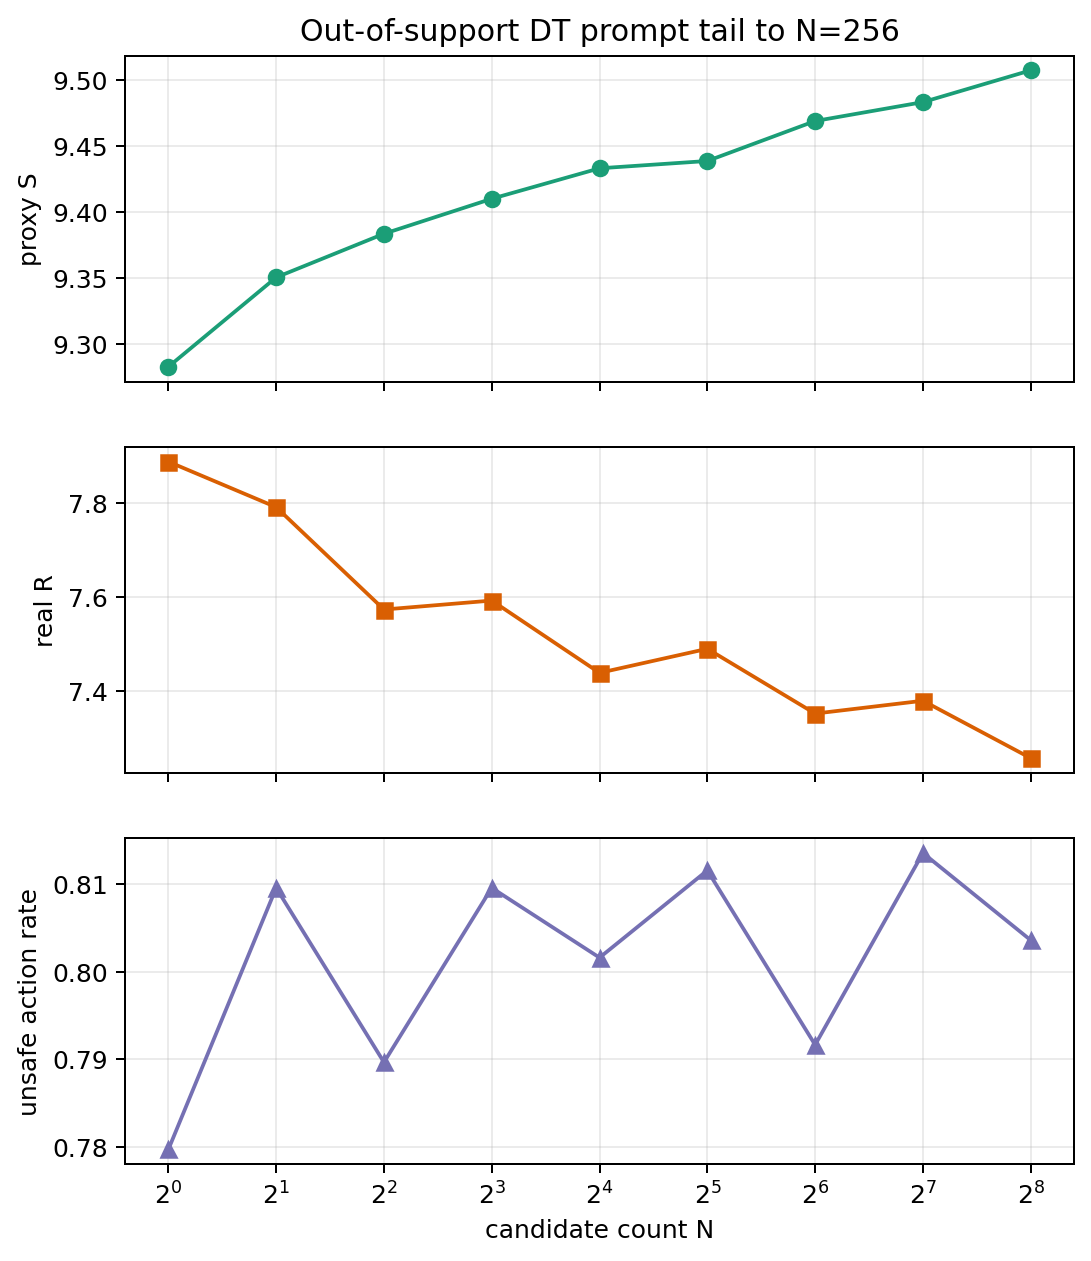
\includegraphics[width=0.92\linewidth]{figures/figure6_candidate_count_256.png}
  \caption{\textbf{$N=256$ candidate-count stress.} Proxy return improves, real utility drops, and selected risk rises as selection pressure moves deeper into the return-support tail.}
  \label{fig:tail256}
\end{figure}

\subsection{Does the exact accounting match Monte Carlo?}

Yes. The exact tie-aware law is evaluated on a finite candidate pool with rounded proxy scores to create ties. Table~\ref{tab:law} reports representative rows. The maximum absolute error in expected real utility across all evaluated $N$ values is $0.00535$, well within one to two Monte Carlo standard errors for the reported rows.

\begin{table}[t]
\centering
\small
\caption{\textbf{Tie-aware accounting validation.} Exact expected real utility closely matches Monte Carlo estimates for top-score selection on the finite candidate distribution.}
\label{tab:law}
\begin{tabular}{rrrrr}
\toprule
$N$ & Exact $\E[\utility]$ & MC $\E[\utility]$ & Abs. error & MC stderr \\
\midrule
1 & 7.879 & 7.878 & 0.00049 & 0.00350 \\
8 & 7.706 & 7.707 & 0.00103 & 0.00386 \\
16 & 7.660 & 7.666 & 0.00534 & 0.00403 \\
64 & 7.516 & 7.520 & 0.00403 & 0.00456 \\
\bottomrule
\end{tabular}
\end{table}

\begin{figure}[t]
  \centering
  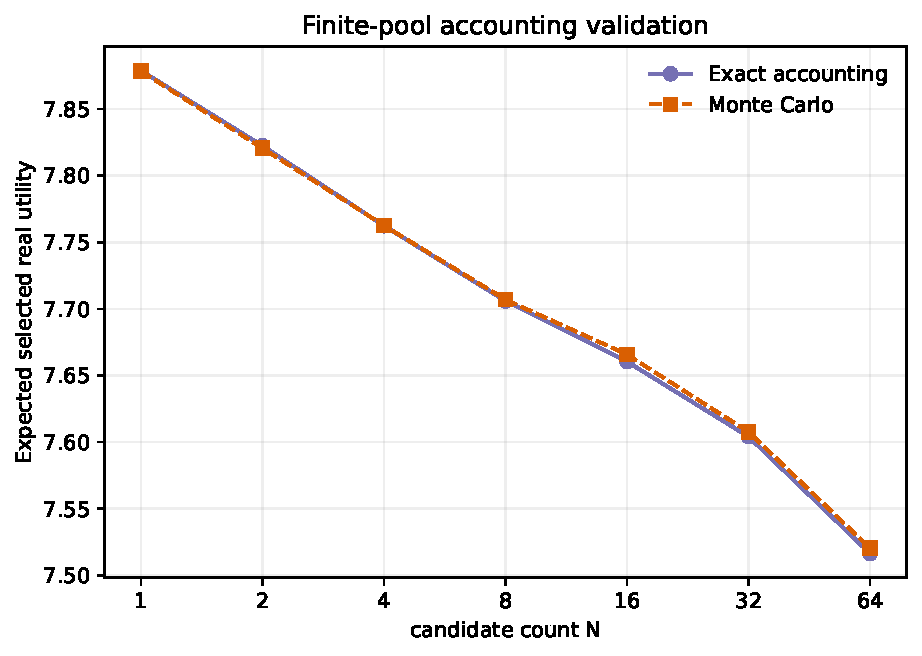
\includegraphics[width=0.90\linewidth]{figures/exact_accounting_validation.pdf}
  \caption{\textbf{Exact accounting validation.} The closed-form finite-pool curve tracks Monte Carlo estimates as selection pressure moves toward the high-score, lower-utility tail.}
  \label{fig:law}
\end{figure}

\subsection{Do support-gap controls behave as predicted?}

The in-support control confirms that candidate-count pressure is not being portrayed as universally harmful. Under the in-support target, naive real utility rises from $4.821$ to $4.975$ between $N=1$ and $N=64$. The edge-support target also improves, from $6.311$ to $6.454$.

The anti-aligned scorer control goes in the opposite direction. We select candidates using a score that is intentionally anti-aligned with real utility under the in-support target. Real utility falls from $4.841$ at $N=1$ to $4.653$ at $N=64$, a change of $-0.188$. This matches Proposition~\ref{prop:law}: increasing $N$ amplifies the high-score tail of whichever score is used.

\begin{figure}[t]
  \centering
  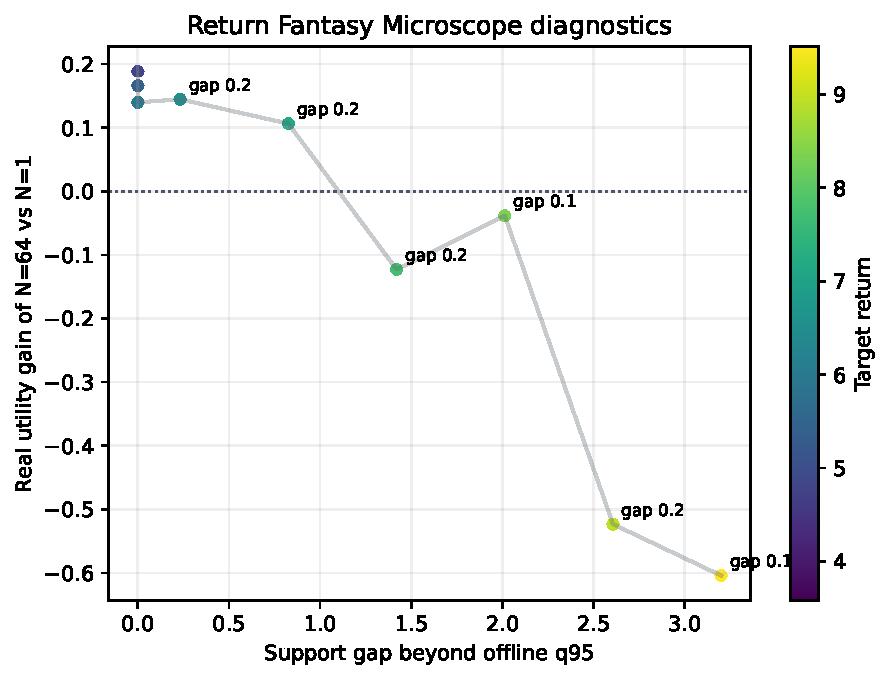
\includegraphics[width=0.86\linewidth]{figures/support_diagnostics.pdf}
  \caption{\textbf{Support diagnostics.} The out-of-support prompt lies beyond the empirical $q_{95}$ and maximum offline proxy-return support. The failure case is therefore an extrapolative target-return condition, not an ordinary supported request.}
  \label{fig:support}
\end{figure}

The expanded target-overshoot sweep makes the boundary sharper. Table~\ref{tab:overshoot} holds $N=256$ fixed and moves the requested return beyond $q_{95}$. At the boundary, $N=256$ selects real utility $6.456$. At $q_{95}+3.0$, the same high-$N$ selection gives $7.362$, but by $q_{95}+4.5$ it collapses to $3.578$ while proxy return continues to track the ambitious prompt. In other words, prompt satisfaction and real utility separate most strongly when the target moves far outside support.

\begin{table}[t]
\centering
\small
\caption{\textbf{Expanded target-overshoot stress at $N=256$.} The support gap is target return minus offline $q_{95}$.}
\label{tab:overshoot}
\begin{tabular}{rrrrrr}
\toprule
Gap & target & proxy $\score$ & real $\utility$ & unsafe rate & support gap \\
\midrule
0.00 & 6.314 & 6.514 & 6.456 & 0.063 & 0.000 \\
0.75 & 7.064 & 7.264 & 7.135 & 0.133 & 0.750 \\
1.50 & 7.814 & 8.011 & 7.629 & 0.310 & 1.500 \\
2.25 & 8.564 & 8.756 & 7.718 & 0.560 & 2.250 \\
3.00 & 9.314 & 9.496 & 7.362 & 0.833 & 3.000 \\
3.75 & 10.064 & 10.241 & 5.893 & 0.925 & 3.750 \\
4.50 & 10.814 & 10.984 & 3.578 & 0.984 & 4.500 \\
\bottomrule
\end{tabular}
\end{table}

\begin{figure}[t]
  \centering
  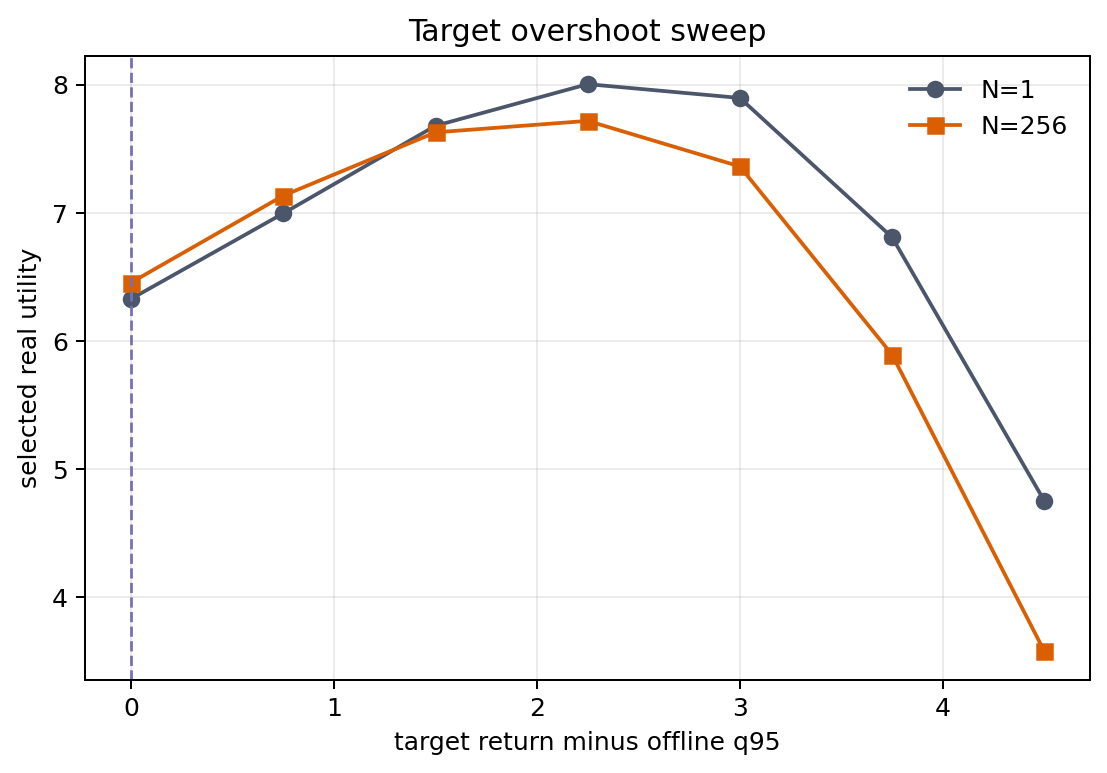
\includegraphics[width=0.90\linewidth]{figures/figure7_target_overshoot.png}
  \caption{\textbf{Target-overshoot stress.} The high-$N$ selector remains prompt-obedient in proxy space, but real utility deteriorates once the requested return is far beyond offline support.}
  \label{fig:overshoot}
\end{figure}

\subsection{Do repairs reduce the failure?}

Table~\ref{tab:repairs} compares the original out-of-support condition at $N=64$. The support-calibrated and conservative-gate rows lower the effective target, dramatically reduce risk, and return candidates closer to the behavior distribution; they should be read as deployment refusals or target reductions, not as attempts to maximize the original high prompt. Likelihood-constrained and pilot-calibrated selection keep the original high-target setting but recover real utility by avoiding the riskiest high-proxy candidates. Pilot calibration improves real utility over naive by $1.009$, close to the oracle diagnostic gain of $1.085$.

\begin{table}[t]
\centering
\small
\caption{\textbf{Original out-of-support repair diagnostics at $N=64$.} Likelihood and pilot repairs recover real utility under the high target. Support and gate repairs mainly reduce off-support pressure and risk.}
\label{tab:repairs}
\begin{tabular}{lrrrr}
\toprule
Strategy & $\score$ & $\utility$ & Risk & $\Delta\utility$ vs naive \\
\midrule
Naive & 9.468 & 7.381 & 0.01739 & 0.000 \\
Support-calibrated & 6.484 & 6.455 & 0.00024 & -0.926 \\
Conservative gate & 5.672 & 5.661 & 0.00009 & -1.720 \\
Likelihood-constrained & 9.217 & 8.457 & 0.00633 & 1.076 \\
Pilot-calibrated & 9.199 & 8.390 & 0.00674 & 1.009 \\
Oracle real & 9.247 & 8.466 & 0.00651 & 1.085 \\
\bottomrule
\end{tabular}
\end{table}

\begin{figure}[t]
  \centering
  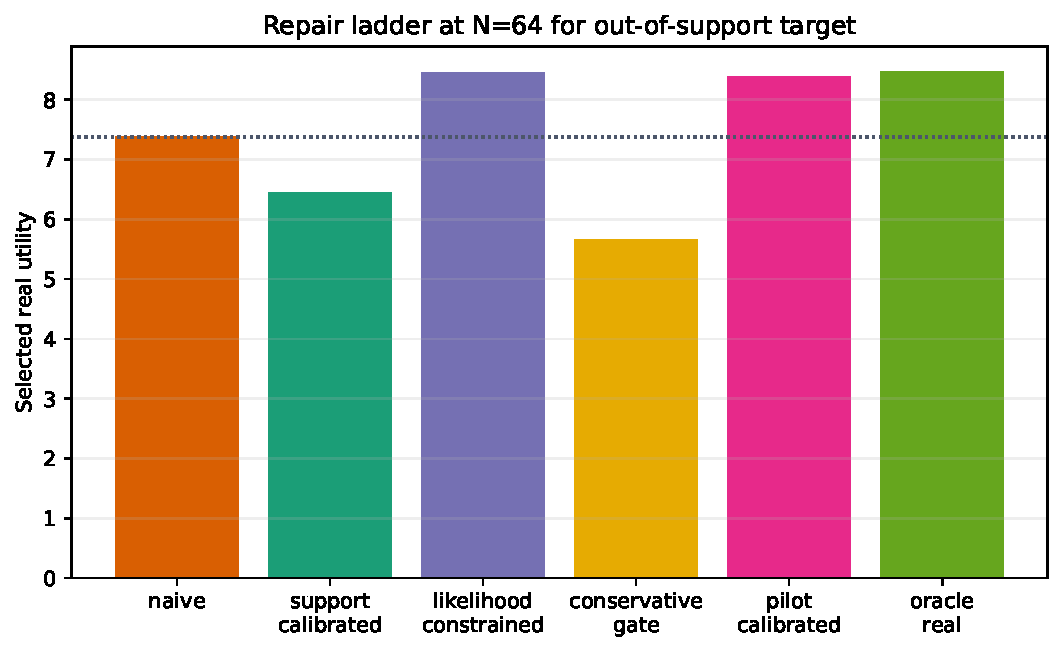
\includegraphics[width=0.92\linewidth]{figures/repair_comparison.pdf}
  \caption{\textbf{Original repair comparison.} Under the out-of-support target, support-aware and utility-aware selectors change the selected tail. The oracle row is a diagnostic upper bound; pilot calibration is the deployable proxy for limited real-utility labels in this study.}
  \label{fig:repair}
\end{figure}

The expanded repair ladder repeats this at $N=256$ and adds support-target reductions, likelihood thresholds, random selection, and an oracle upper bound. Table~\ref{tab:repair256} reports the high-candidate rows. Raw selection obtains real utility $7.303$. Behavior-likelihood filtering recovers $1.216$ real-utility points, pilot calibration recovers $1.146$, and the oracle diagnostic gap is $1.239$. The support-calibrated rows lower the target and reduce risk, so they are not direct wins over raw high-target utility; they are evidence that a support-aware deployment gate should ask for a lower prompt or real labels instead of blindly increasing $N$.

\begin{table}[t]
\centering
\small
\caption{\textbf{Expanded repair ladder at $N=256$.}}
\label{tab:repair256}
\begin{tabular}{lrrrrr}
\toprule
Selector & proxy $\score$ & real $\utility$ & risk & unsafe rate & behavior logp \\
\midrule
Random & 9.287 & 7.885 & 0.0117 & 0.784 & -4.847 \\
Naive & 9.501 & 7.303 & 0.0183 & 0.794 & -5.415 \\
Naive q90 & 5.701 & 5.695 & 0.00005 & 0.016 & 0.161 \\
Naive q95 & 6.519 & 6.491 & 0.00023 & 0.044 & -0.546 \\
Behavior q10 & 9.207 & 8.512 & 0.0058 & 0.933 & -4.522 \\
Behavior q05 & 9.195 & 8.519 & 0.0056 & 0.915 & -4.497 \\
Pilot-calibrated & 9.173 & 8.449 & 0.0060 & 0.897 & -4.472 \\
Oracle real & 9.237 & 8.542 & 0.0058 & 0.940 & -4.574 \\
\bottomrule
\end{tabular}
\end{table}

\begin{figure}[t]
  \centering
  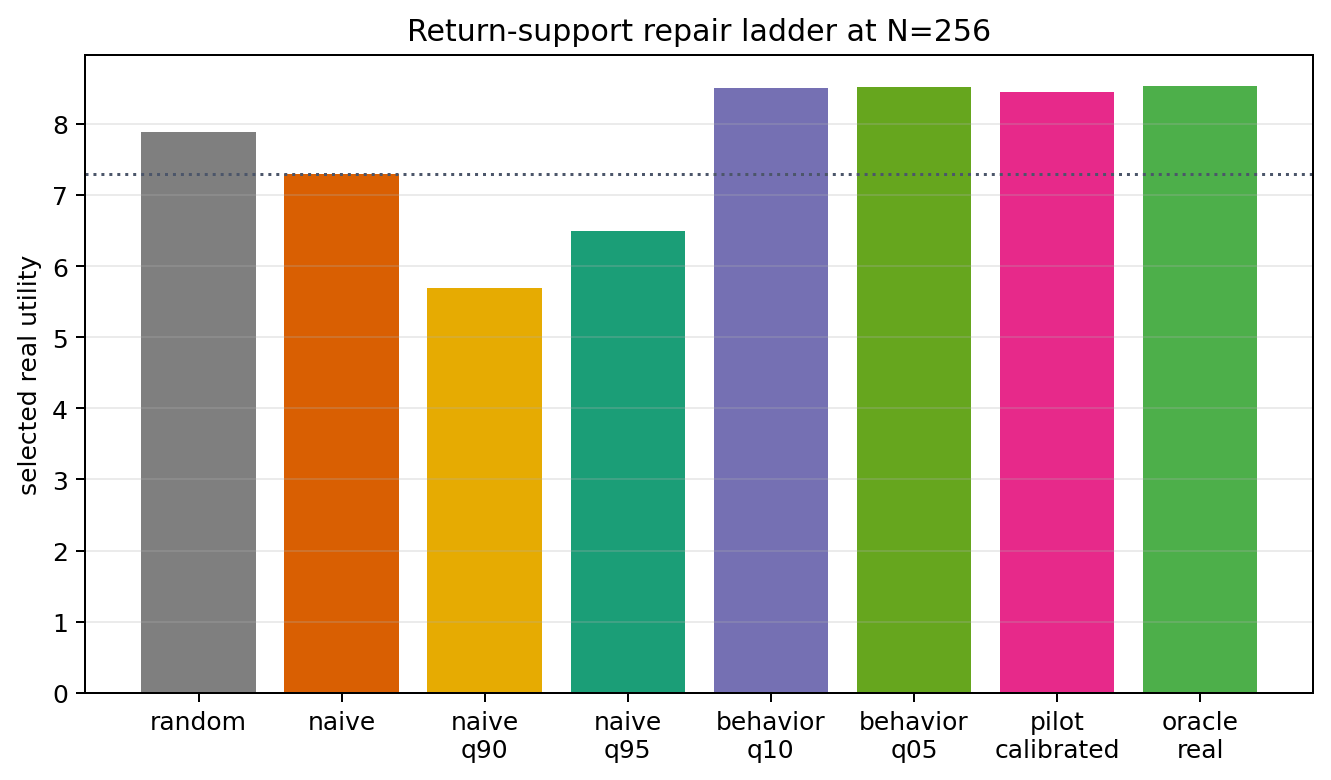
\includegraphics[width=0.92\linewidth]{figures/figure8_repair_ladder_256.png}
  \caption{\textbf{Expanded repair ladder at $N=256$.} Likelihood and pilot repairs select lower-risk, higher-real-utility trajectories from the same high-return candidate pool.}
  \label{fig:repair256}
\end{figure}

\subsection{How sensitive are repairs to pilot labels and rollout noise?}

The v3 suite attacks two practical knobs. First, pilot calibration depends on a small set of real-utility labels. Table~\ref{tab:pilot} varies the pilot set at $N=256$. Four labels already improve over raw high-$N$ selection, but more labels stabilize the calibrator and raise real utility above $8.5$ in the $32$ and $64$ label settings.

\begin{table}[t]
\centering
\small
\caption{\textbf{Pilot-label budget ablation at $N=256$.}}
\label{tab:pilot}
\begin{tabular}{rrrrr}
\toprule
Pilot labels & proxy $\score$ & real $\utility$ & risk & behavior logp \\
\midrule
4 & 9.225 & 8.077 & 0.0096 & -4.681 \\
8 & 9.174 & 8.369 & 0.0067 & -4.496 \\
16 & 9.187 & 8.453 & 0.0061 & -4.499 \\
32 & 9.185 & 8.517 & 0.0056 & -4.479 \\
64 & 9.218 & 8.520 & 0.0058 & -4.541 \\
\bottomrule
\end{tabular}
\end{table}

Second, rollout noise changes how much tail mass is available to selection. Table~\ref{tab:noise} shows $N=256$ naive selection under four noise scales. Larger noise creates higher proxy-return tails but also higher selected risk and lower real utility. This is a DT-specific version of a familiar inference-time lesson: more stochastic search is not free when the score rewards unsupported extrapolation.

\begin{table}[t]
\centering
\small
\caption{\textbf{Rollout-noise stress at $N=256$.}}
\label{tab:noise}
\begin{tabular}{rrrrr}
\toprule
Noise scale & proxy $\score$ & real $\utility$ & risk & unsafe rate \\
\midrule
0.16 & 9.468 & 7.612 & 0.0155 & 0.857 \\
0.32 & 9.499 & 7.186 & 0.0193 & 0.796 \\
0.48 & 9.530 & 6.870 & 0.0222 & 0.770 \\
0.64 & 9.571 & 6.217 & 0.0279 & 0.744 \\
\bottomrule
\end{tabular}
\end{table}

\begin{figure}[t]
  \centering
  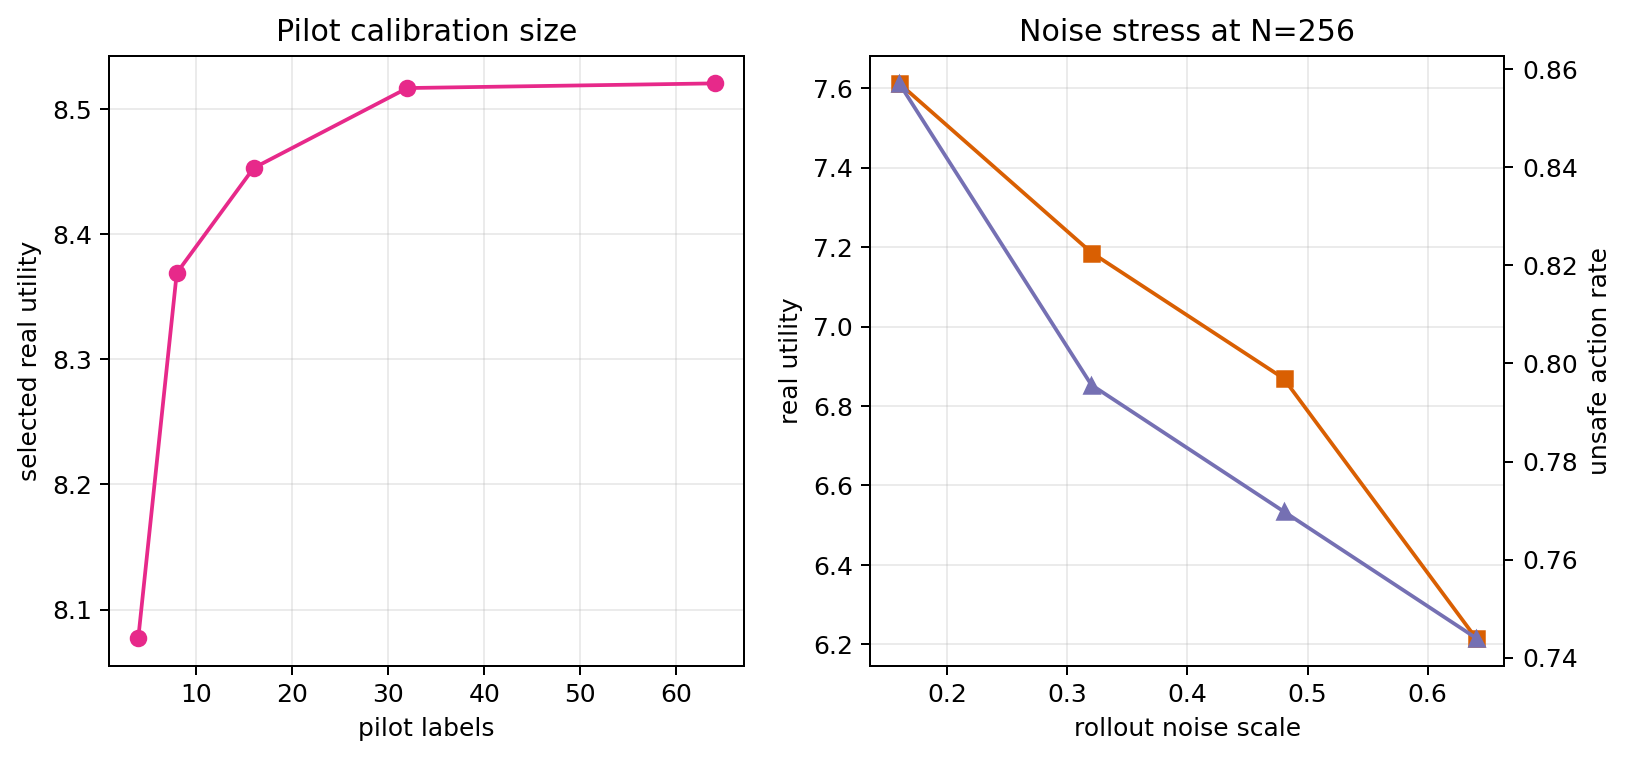
\includegraphics[width=0.94\linewidth]{figures/figure9_pilot_noise_stress.png}
  \caption{\textbf{Pilot and noise stress.} More pilot labels improve calibrated real utility, while higher rollout noise deepens the raw high-score tail and reduces real utility.}
  \label{fig:pilot-noise}
\end{figure}

\paragraph{Claim audit.}
The repository audit returns the verdict \texttt{submission-ready v3} only when the original suite, expanded suite, forbidden-claim scan, and final 25-page PDF check pass. The supported claims are exactly the controlled claims tested here: finite-pool accounting validation, out-of-support fantasy detection, support-gap controls, anti-aligned scorer behavior, repair diagnostics, deployment-gate validity, expanded $N=256$ stress, and absence of overbroad offline-RL claims.
